% Vertical Line Title Page
% LaTeX Template
% Version 2.0 (22/7/17)
%
% This template was downloaded from:
% http://www.LaTeXTemplates.com
%
% Original author:
% Peter Wilson (herries.press@earthlink.net) with modifications by:
% Vel (vel@latextemplates.com)
%
% License:
% CC BY-NC-SA 3.0 (http://creativecommons.org/licenses/by-nc-sa/3.0/)

\documentclass{article}
\usepackage[utf8]{inputenc}
\usepackage{hyperref}
\usepackage{graphicx}

\usepackage{sectsty}
\usepackage{xcolor}

\sectionfont{\color{pink}}
\subsectionfont{\color{blue}}
\subsubsectionfont{\color{cyan}}


\begin{document}
%---------------------------------------------------------------------------------
%	TITLE PAGE
%--------------------------------------------------------------------------------

\begin{titlepage} % Suppresses displaying the page number on the title page and the subsequent page counts as page 1
	
	\raggedleft % Right align the title page
	
	\rule{1pt}{\textheight} % Vertical line
	\hspace{0.05\textwidth} % Whitespace between the vertical line and title page text
	\parbox[b]{0.75\textwidth}{ % Paragraph box for holding the title page text, adjust the width to move the title page left or right on the page
		
		{\Huge\bfseries Elaboration \\[0.5\baselineskip] Assignment}\\[2\baselineskip] % Title
		{\large\textit{Planning and Testing}}\\[4\baselineskip] % Subtitle or further description
		{\Large\textsc{Emily Hunt 44888619}} % Author name, lower case for consistent small caps
		
		\vspace{0.5\textheight} % Whitespace between the title block and the publisher
		}

\end{titlepage}


View in Overleaf: \url{https://www.overleaf.com/read/bkhpthjqbtdr}

\tableofcontents

\pagebreak

\section{Scoping II Decomposition}
I realised I partially misunderstood the expectation for decomposition last week (my response for this section was more appropriate for the algorithm section). So I will first re-attempt decomposition, by breaking down my usual process for analysing the colour of films.

\begin{enumerate}
    \item I watch a film in its entirety taking notes on the colour palette used and how various colours are used thematically. These will most likely \textbf{not} be labelled very clearly (e.g. with time stamps) but just be general notes.
    \item When reviewing these notes to write an essay etc., I will have to go back through the film and try and work out which part of it the notes are referencing, which can be a very time consuming and fiddly process.
\end{enumerate} 

Using the XY Problem resource (\url{http://xyproblem.info/}), I also realised that my issue was not solely analysing the colour of films, but organising my notes concerning these. Therefore, the technologies listed below to accomplish each step in the decomposition will be divided into those that assist with colour analysis, and note taking. These will be evaluated in terms of what Brian noted on Slack to be signs of a good tool (well written and easily understandable documentation, as well as recent maintenance (indicating wide use)).

\section{PLANNING}

\subsection{Solutions for Colour Analysis}
I couldn't really find a tool that did specifically what I identified in scoping (measures the number of times a colour appears throughout a film), so I switched my focus to tools that would create a colour map of a film.

\subsubsection{GitHub: Cinemetrics (Original)}
URL: \url{https://github.com/freder/cinemetrics}\\

This tool would be ideal, as in addition to producing a map of the colours present in a film, it provides a representation of a number of the film's other features, such as shot duration and motion, which are things I hadn't really considered before. However, this tool will probably not be viable to use, as it fails to meed a number of the criteria identified on Slack: 
\begin{itemize}
    \item Documentation: There is no documentation provided with this tool, as explicitly noted on its GitHub repository.
    \item Maintenance: The last commits for this project were 8/9 years ago.
\end{itemize}

\subsubsection{GitHub: Cinemetrics}
URL: \url{https://github.com/suite22/cinemetrics}\\

This tool is a different version of the previously identified one. It seems more feasible than the other option in one respect:

\begin{itemize}
    \item Documentation: Detailed documentation is provided with this tool. From a preliminary reading, it seems to be understandable.
    \item Maintenance: However, similarly to the aforementioned tool, a number of the latest commits for a number of the files were 8 years ago, though a few were as recent as 3/4 years ago.
\end{itemize}
I did an initial test of this software. I installed vagrant as instructed, downloaded a zip of the repository and then in Terminal, made the copy of the repository the working directory and entered 'vagrant up'. This produced a message informing me I needed to install a 'provider', with VirtualBox recommended. However, I had some issues with security and privacy settings when trying to install VirtualBox, so stopped the test here. I have recorded my actions in more detail in the testing section.

\subsubsection{GitHub: Colors-of-Film}
URL: \url{https://github.com/sacert/Colors-of-Film}\\

This tool may also prove to be a viable option. It allows customisation of the size (length/width) of the output colour map image.
\begin{itemize}
    \item Documentation: The documentation is very straightforward and clear, and it seems the software is simple to use.
    \item Maintenance: The last commits were 2/3 years ago, and the repository has 16 stars.
\end{itemize}

\subsubsection{GitHub: FilmStrip}
URL: \url{https://github.com/ArkadiusBear/FilmStrip}\\

The tool may also be viable for producing a colour map of a film. At allows the customisation of a number of aspects of the output image, including size, ratio and density.

\begin{itemize}
    \item Documentation: Really clear documentation is provided regarding what the tool does and how it works, though there doesn't appear to be much documentation in relation to how to use the tool.
    \item Maintenance: The last commits were 8 months ago, making this the most recently updated repository of all the tools listed. However, these commits were only over two days, indicating there has not been a long process of testing and updating.
\end{itemize}
 
\subsection{Solution for Note Taking: ClipNotes}
URL: \url{http://www.clipnotes.org/}\\

Though I can't locate the code for this tool, it seems like it could be a really valuable tool. It appears that for it to work, you download the app, have a film file and your notes (with a time stamp) in an XML file. You can then open the film file and notes in the app, and it will display the notes at the appropriate time in the film.
\begin{itemize}
    \item Documentation: There is really detailed documentation on how to use the software on the website, as well as a trouble shooting section.
    \item Maintenance: From what I can see, the last update of the software was 2015.
\end{itemize}

This solution could be potentially combined with one of the colour analysis solutions, so that a specific portion of the colour map could be linked (through the XML file?) to that specific section of the film if I want to view it in more detail.

\subsection{Inspiration}

The inspiration for the potential combination for these two tools came from an app called 'Animated' by Walt Disney Animation Studios. It includes a colour map of each of the studio's films which you can select and scrub through to see certain stills. While this is useful to me in its current form (as I plan to analyse Disney films in my thesis) the production of colour maps is something I would like to learn how to do for potential future studies. Furthermore, in their current form the colour maps in this app are difficult to navigate as it is really fiddly to select and scrub through a specific film. I would like to be able to have a colour map and go that section of the film to look at in more detail, while also being able to see the notes I have written, which is what I am proposing in this elaboration.


\pagebreak

\section{TESTING}

To test each of these solutions that required a video file, I used a 3 minute video I had taken on my iPhone of a parade. This was chosen because I thought using a smaller video file (rather than a full length film) would allow me to test the solutions more quickly, and I still have to think about sourcing the full length films and potential copyright considerations. I also placed a one hour limit on the tests for each of the different tools. They were not tested in the order they are listed which may be reflected in the time stamps.

\subsection{Solutions for Colour Analysis}

\subsubsection{GitHub: Cinemetrics}
URL: \url{https://github.com/suite22/cinemetrics}\\

As noted in planning, this tool lacked proper documentation so I was unable to test it. I instead focused on just testing the next tool which is a version of this one.

\subsubsection{GitHub: Cinemetrics}
URL: \url{https://github.com/suite22/cinemetrics}\\

As noted in the Elaboration Plan submitted to CloudStor, I did an initial test of this tool last week. However, I forgot to log this in my learning journal, so have noted my actions here but do not have the appropriate time stamps for a number of the steps.\\

\textbf{Objective: Install Vagrant}\\
\textbf{Actions:} As the GitHub Repository for this tool noted Vagrant was a requirement, I followed the link it provided to install it (\url{https://www.vagrantup.com/}. On this page, I selected the Download 2.2.5 button. I then selected the mac0S 64 bit option, with this automatically starting the download. Once it downloaded, I opened the file, and then selected vagrant.pkg and followed the prompts to install it.  \\
\textbf{Results:} Vagrant seemed to successfully install.\\
\textbf{Errors:} None.\\
\textbf{Solutions/Notes:}\\

\textbf{Objective: Download a Repository from GitHub}\\
\textbf{Actions:} In the main page of the GitHub repository I clicked on the green Clone or Download button. I then selected Download Zip. Once the zip had downloaded, I unzipped it and saved the folder to my desktop.\\
\textbf{Results:} This successfully saved the contents of the repository to my folder.\\
\textbf{Errors:} None\\
\textbf{Solutions/Notes:}\\

\textbf{Objective: Attempt to Run the Python Files by Following the Instructions on GitHub}\\
\textbf{Actions:} I opened Terminal, and made the folder downloaded from GitHub my working directory. As instructed I entered 'vagrant up'.\\
\textbf{Results/Errors:} I received the message below.
\begin{figure}[htp]
    \centering
    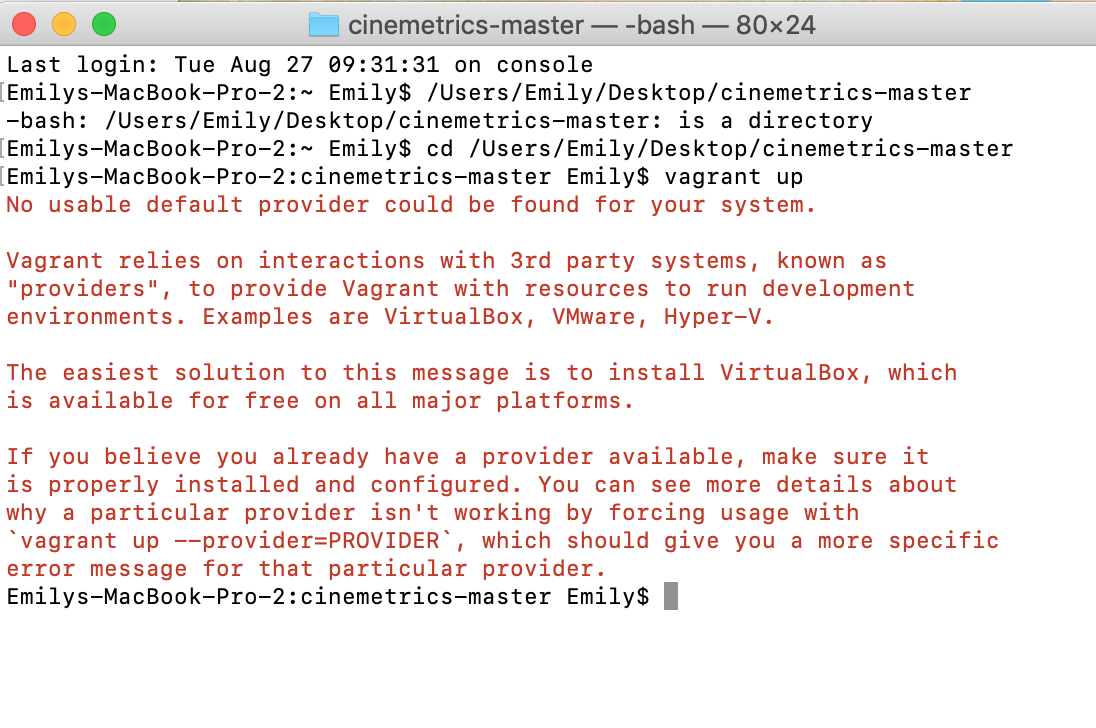
\includegraphics[width=12cm]{Vagrant_Image_1.png}
    \caption{Error 1 When Attempting to Run Vagrant}
\end{figure}

\textbf{Objective: Address the Error Message by Installing VirtualBox}\\
\textbf{Actions:} I searched VirtualBox on Google which led me to this site \url{https://www.virtualbox.org}. I clicked the large Download VirtualBox 6.0 button, and on the page this took me to, under VirtualBox 6.0.12 platform packages selected OS X hosts which began the download. Once the download had completed, I again followed the prompts to install the software.\\
\textbf{Results/Errors:} At the final stage of installation I received an error message that my security and privacy settings would not allow the app to be installed. \\
\textbf{Solutions/Notes:} However, after testing some of the other solutions which required me to adjust my settings, VirtualBox opened successfully.\\

\textbf{Objective: Second Attempt to Run the Python Files by Following the Instructions on GitHub}\\
\textbf{Time Stamp:} 9:30pm 4 September\\
\textbf{Actions:} I again entered 'vagrant up' in the correct directory in Terminal.\\
\textbf{Results/Errors:} I now received the message below\\
\begin{figure}[htp]
    \centering
    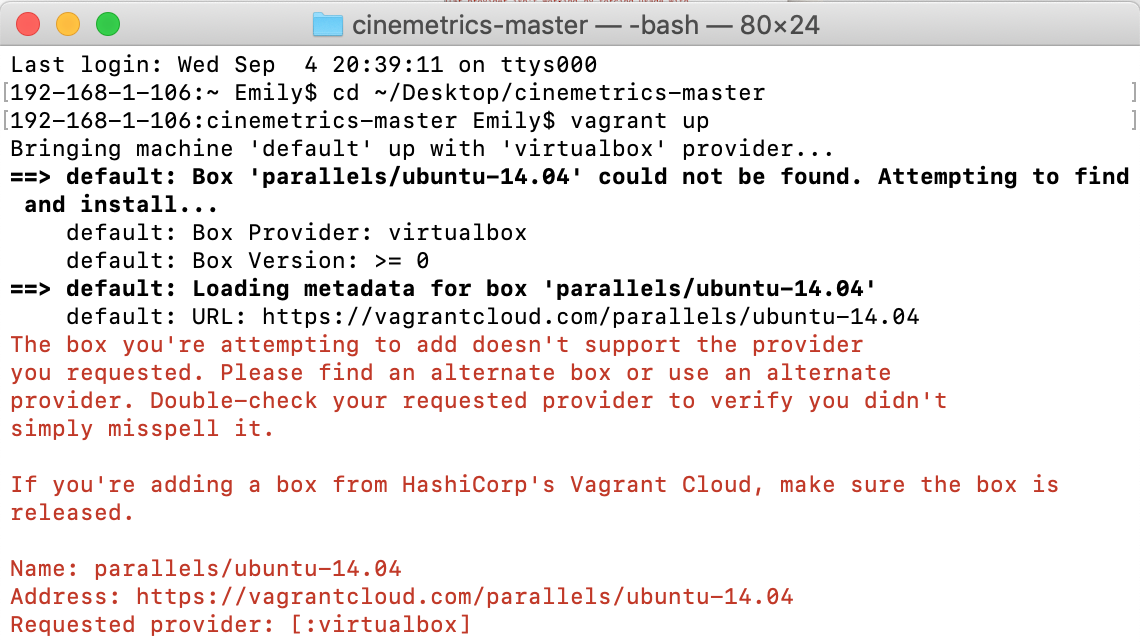
\includegraphics[width=12cm]{Vagrant_Image_2.png}
    \caption{Error 2 When Attempting to Run Vagrant}
\end{figure}

\textbf{Solutions/Notes:} I searched online for solutions and the most common one was to enter 'vagrant up --provider virtualbox', but this presented the same message. When returning to this document to record my tests, I went to the Vagrant website to copy the URL. I noticed in the image on the main page, prior to 'vagrant up' was 'vagrant init hashicorp/precise64'. So I tried entering this first and this successfully opened vagrant. The shell informed me though that I had to delete the existing Vagrantfile in the directory, which I did, and then I reran the command. I then entered 'vagrant up' which printed some text and had a progress percentage. I ended up terminating the shell because I wanted to have a better understanding of what Vagrant actually did before I ran it.\\

\subsubsection{GitHub: Colors-of-Film}
URL: \url{https://github.com/sacert/Colors-of-Film}\\

\textbf{Objective: Try Running the Python Script}\\
\textbf{Time Stamp:} 11:45am 3 September\\
\textbf{Actions:} The information on the GitHub page said I needed Numpy and OpenCV, but I wanted to just see what happened if I tried to run it. I downloaded the GitHub Repository as a zip, unzipped the folder and moved it to my desktop. I then moved the file I wanted to trial the python script on into the folder using GUI, and then made this the working directory in the Unix Shell. As instructed, I entered, 'python colorsOfFilm.py Test.mov 50 30'.\\
\textbf{Errors:} This produced the message 'File "colorsOfFilm.py", line 2, in \textless{} module \textgreater{}; import cv2;ImportError: No module named cv2'.\\
\textbf{Solutions/Notes:} I then tried to install OpenCV.\\

\textbf{Objective: Install OpenCV}\\
\textbf{Time Stamp:} 12:06pm 3 September\\
\textbf{Actions:} I went to \url{https://opencv.org/} and clicked learn more under 'OpenCV 4.1.1 The latest release is now available'. Under OpenCV – 4.1.1, I clicked iOS pack, which took me to SourceForge where a zip file started automatically downloading. I unzipped the file named 'opencv2.framework' and moved it to the folder I had downloaded from GitHub and attempted to run the python script again using the same input into Terminal. \\
\textbf{Results/Errors:} The same error message appeared.\\
\textbf{Solutions/Notes:} I then searched online for how to install OpenCV. One of the common solutions was variations of entering 'pip install opencv'. However, this produced the response '-bash: pip: command not found'. Searching for a solution took me to the end of the hour I allotted from testing meaning I had to conclude the test at this point. If I return to this, the next step after resolving this error would be to install NumPy. To do so, see this website \url{https://numpy.org/}.\\

\subsubsection{GitHub: FilmStrip}
URL: \url{https://github.com/ArkadiusBear/FilmStrip}\\

\textbf{Objective: Attempt to Run the Script}\\
\textbf{Time Stamp:} 10:30pm 4 September\\
\textbf{Actions:} I downloaded the repository from GitHub and made it the working directory in Terminal. I entered a similar command to what was suggested from the previous tool - 'python FilmStrip.ps1 Test.mov'\\
\textbf{Results/Errors:} This printed the response, 'File "FilmStrip.ps1", line 3; [Parameter(Mandatory=\$true)];SyntaxError: invalid syntax\\
\textbf{Solutions/Notes:} After some searching online, I realised a ps1 file is for Windows PowerShell, where I am working on a mac.\\

\textbf{Objective: Install PowerShell}\\
\textbf{Time Stamp:} 10:40pm 4 September\\
\textbf{Actions:} After some googling, I found that you can install PowerShell on a mac. At this site \url{https://docs.microsoft.com/en-us/powershell/scripting/install/installing-powershell?view=powershell-6}, I clicked on Installing PowerShell Core on macOS. On the page this took me to, I went down to Installation via Direct Download, and clicked on the link to the releases page and clicked on powershell-6.2.2-osx-x64.pkg which started the automatic download. I then clicked on the file and followed the prompts to install the program.\\
\textbf{Results:} I searched PowerShell in Finder, clicked on the app and it opened successfully.\\
\textbf{Errors:} None.\\
\textbf{Solutions/Notes:} \\

\textbf{Objective: Run the ps1 File in PowerShell}\\
\textbf{Time Stamp:} 10:50pm 4 September\\
\textbf{Actions:} In PowerShell, I made the folder downloaded from GitHub the working directory using the same process as in Terminal. Using this site about running a PowerShell script to help me, \url{https://www.dummies.com/computers/operating-systems/windows-xp-vista/create-run-powershell-script/}, I entered './FilmStrip.ps1 ./Test.mov' in Powershell. \\
\textbf{Results/Errors:} This printed a lot of red text, with Invalid Operation appearing frequently. It took about 30 seconds to finish printing (this was only a 3 minute video so the length of time it takes to process an entire film may be prohibitive).\\
\textbf{Solutions/Notes:} I need to do more research into how to write a command in PowerShell and may go to consultation hours.\\

\subsection{Solution for Note Taking: ClipNotes}
URL: \url{http://www.clipnotes.org/}\\

\textbf{Objective: Download ClipNotes App to My iPad}\\
\textbf{Time Stamp:} 1:35pm 3 September\\
\textbf{Actions:} On my iPad, I went into the App Store and searched Clip Notes. I clicked GET and then INSTALL on the appropriate app (the icon with the film strip down the middle and a paper clip).\\
\textbf{Results:} The app was installed successfully. I opened the app and viewed the example film and notes. If you clicked on a specific note, it was expanded under the viewing window and it played the specific part of the film the note referred to, stopping at the end timestamp. You select Change Film to switch to a different film you have saved to the app or Change Notes to different notes you have saved. As I didn't have another film or notes I couldn't change these.\\
\textbf{Errors:} None.\\
\textbf{Solutions/Notes:} You cannot use films saved to your iPad in iTunes, you have to save them to the app from iTunes on your computer (as it says on the site).\\

\textbf{Objective: Create a XML File with My Notes}\\
\textbf{Time Stamp:} 1:45pm 3 September\\
\textbf{Actions:} I checked the ClipNotes website and TextWrangler which I already had installed on my computer was listed as an XML editor to use. So I created a file with notes for two sections of the film (with a caption and description) using the template from the ClipNotes site, and saved the file on my desktop.\\
\textbf{Results:} The file was successfully saved, but as a .txt file, which caused me issues later. \\
\textbf{Errors:} I encountered an error when trying to open this file in the app. \\
\textbf{Solutions/Notes:} Please see Error: Notes File Causing the App to Crash on page \pageref{crash} for solutions to this error.\\

\textbf{Objective: Transfer Video and Notes Files to iPad from Computer}\\
\textbf{Time Stamp:} 1:52pm 3 September\\
\textbf{Actions:} I connected my iPad to my computer using a lightning to USB cable. iTunes opened automatically, and I selected the iPad symbol near the top menu bar. In the page this opened, in the left menu bar I selected 'File Sharing' (it has the little 'A' symbol next to it like the App Store logo). Under Apps, I selected ClipNotes, and dragged and dropped the appropriate files into the space for files (I could have also clicked the Add button).\\
\textbf{Results:} These were successfully transferred onto my iPad after a short period.\\
\textbf{Errors:} None. \\
\textbf{Solutions/Notes:}\\

\textbf{Objective: Open Video and Notes in App}\\
\textbf{Time Stamp:} 2:00pm 3 September\\
\textbf{Actions/Results:} Within the app, I selected Change Film. The one I had transferred to my iPad appearred, I selected it and it was successfully loaded in the viewing window.\\
\textbf{Errors:} However, when I selected Change Notes, the app crashed. When I quit the app and then tried to reopen it the app would not open at all.\\
\textbf{Solutions/Notes:} Please see the next Error.\\

\textbf{Error: Notes File Causing the App to Crash}\label{crash}\\
\textbf{Actions:} I realised my issue was a result of the file not being in an XML format. After some searching online, the most frequently suggested solution to my problem was, within TextWrangler, selecting Text in the menu bar, and then Apply Text Filter. However, TextWrangler would not allow me to select this option. I then tried creating an XML file from the Unix Shell, by entering 'nano test.xml' with the Desktop as my working directory. When transfered to my iPad, this still caused the app to crash. I also tried just changing the extension of the file from .txt to .xml which didn't work either (I know we were told not to do this in class but I wanted to exhaust all options). I then looked at the Troubleshooting section of the ClipNotes website which informed me a common problem is issues in the XML files (such as not correctly closing a tag). From this, I realised I had not correctly closed my main \verb|<\Clips>| tag. I then addressed this issue in the file I had created in the Unix Shell but this still caused the app to crash. I then went to the XML Database of film notes on the ClipNotes website. I selected the notes for the film \textit{Contempt} (A random choice) which opened in a new tab. I then selected File in the menu tab and selected Save. In the window that opened, the format of the file was 'XML text'. I saved the file to my desktop and transferred it to my iPad. The app opened and the notes for the film opened successfully with the video I had transferred. On my computer, I then edited the \textit{Contempt} notes file to be notes for my own video, and then transferred this to my iPad, and these opened successfully with the video on the app, playing the correct portions of the video with the corresponding notes.

\subsection{Solution for Script Analysis: ScriptThreads}
During my research into ClipNotes, I found this article (\href{http://www.teachingmedia.org/clipnotes-in-the-classroom-video-annotation-software-for-instruction-and-collaboration/}{Click Here}) discussing ScriptNotes which notes other Digital Humanities tools and resources for the Cinema and Media Studies. \\
This article mentions the tool ScriptThreads.\\

URL: \url{http://www.scripthreads.org/}\\

\textbf{Objective: Install and Open the ScriptThreads Application on My Computer}\\
\textbf{Time Stamp:} 9:30pm 3 September\\
\textbf{Actions:} On the ScriptThreads website, I went to the download tab and under ScriptThreads prototype clicked the link for the Mac OSX 64 version of the software. This started automatically downloading a zip folder. Once the file had finished downloading, I unzipped the file. In the unzipped folder, I selected the ScriptThreads application to open the file.\\
\textbf{Results:} See Errors.\\
\textbf{Errors:} At first the app wouldn't open as my security settings wouldn't allow me to open an app not downloaded from the App Store or a know developer.\\
\textbf{Solutions/Notes:} I went into System Preferences, and went to Security and Privacy. In the apps downloaded from section, ScriptThreads appeared and it said Open Anyway. I selected this and then confirmed I wanted to open it even though it wasn't from a known developer. The app then successfully opened. When it opens, a pop up appears asking if I want to create sample breakstring file as no breakstring file was found (I selected OK). An information pop-up then appears for the app, I selected OK and it opened successfully. \\

\textbf{Objective: Find a Film Script in HTML Format}\\
\textbf{Time Stamp:} 9:38pm 3 September\\
\textbf{Actions:} In order to breakdown a script, the app requires a script in HTML format. For this test, I went to the site \url{https://www.dailyscript.com/} and selected the first script under the Movie Scripts tab (\textit{10 Things I Hate About You}). I then went to the File in the menu bar, selected Save As ..., made sure the file was saving in HTML format and saved the script to my desktop.\\
\textbf{Results:} The file was saved successfully in the correct format.\\
\textbf{Errors:} None.\\
\textbf{Solutions/Notes:} In future, copyright considerations may need to be taken into account.\\

\textbf{Objective: Open the Downloaded Script in the App}\\
\textbf{Time Stamp:} 9:47pm 3 September\\
\textbf{Actions:} In the ScriptThreas app I went to File, Open File and then selected the \textit{10 Things I Hate About You} script. This then brought up a progress bar that the script was parsing.\\
\textbf{Results:} A graphical representation of the script was produced. I played around with the settings in the left menu bar to see what changes they would make. The app identified changes in the scene really well, as it would highlight alternate ones gray.\\
\textbf{Errors:} However, the app had taken random letters from the file to be the characters, and not the actual character names. I tried to address this problem in the next objective.\\

\textbf{Objective: Make ScriptThreads Identify Specific Character Names}\\
\textbf{Time Stamp:} 10:00pm 3 September\\
\textbf{Actions:} Firstly, I duplicated the \textit{10 Things I Hate About You} script, and made a short mock up script of my own, using EMILY as a character and scene location descriptions which included (INT or EXT). I then opened my new test file in ScriptThreads and it successfully highlighted the alternate scenes and identified the scene descriptions (highlighting them in purple). Then in the top menu bar I went to Characters and selected Force Character, this produced a pop up titled Included Characters. In the bottom left hand corner I clicked the + button, and was prompted to enter a character name. I entered EMILY and clicked OK. I then chose a random source colour for the character on a colour wheel (blue) and clicked OK, closing the pop up. I then selected File, Reparse in the menu bar.\\
\textbf{Results:} See Errors.\\
\textbf{Errors:} This did not have any effect on the script.\\
\textbf{Solutions/Notes:} I then looked through the different options in the menu bar. Under Options I selected Parsings. In this pop up I deselected Find Characters in the Text and selected OK. I then tried reparsing the file again, and this produced a single line down the centre of the graph image in blue and EMILY was highlighted in the correct colour in the script.\\

\section{Thinking to the Future}
I am hoping ScriptThreads may be a viable, as well as educationally valuable, option for the Proof of Concept. For a project I am completing in another unit, I am comparing the films \textit{Snow White and the Seven Dwarfs} (1937) and \textit{The Little Mermaid} (1989). When I look online for the scripts for these films, they are not in a form that can be read by the tool (e.g. The lines are just denoted by time stamps and not characters). I could potentially clean this data for use by the tool and then process it with ScriptThreads. However, copyright issues is something I need to consider moving forward.\\

Another tool I found since completing the Elaboration 1 Planning exercise was the ACTION-Video-Toolkit (\url{https://github.com/bregmanstudio/ACTION-Video-Toolkit}). This tool would be absolutely ideal for my completing my thesis, as it supposedly provides a toolkit to analyse similarities across films. I consulted Brian on Slack and he expressed some concerns over the tool and pointed me in the direction of a GitHub repository for switching between different versions of Python in order to use the version that this tool was created on (\url{https://github.com/pyenv/pyenv}). Unfortunately, as a result of time costs, I was unable to test this tool for this task. However, I wanted to make a note of it here for potential future reference.\\

\end{document}